\documentclass[a4paper,11pt,notitlepage,fullpage]{article}
%\documentclass{report}

\usepackage{fullpage}
\usepackage[utf8]{inputenc}
\usepackage[ngerman]{babel}
%\usepackage[english]{babel}
\usepackage{amsmath}
\usepackage{amssymb}
\usepackage{latexsym}
\usepackage{mathtools}
\usepackage{listings}
\usepackage{bbm}
%\usepackage{algorithm}
%\usepackage{algpseudocode}
\usepackage{graphicx}
\usepackage{booktabs}
\usepackage{hhline}
\usepackage{amsthm}
\usepackage{cite}
\usepackage{wrapfig}
\usepackage{hyperref}
\usepackage{titling}
\usepackage{color}

\setlength{\droptitle}{-60pt}

\newcommand{\R}{\mathbb R}
\newcommand{\N}{\mathbb N}

\newcommand{\p}{\mathbb P}
\newcommand{\pp}[1]{\mathbb P\left[#1\right]}
\newcommand{\ppp}[2]{\mathbb P_#1\left[#2\right]}
\newcommand{\E}{\mathbb E}
\newcommand{\Ee}[1]{\mathbb E\left[#1\right]}
\newcommand{\V}{\mathbb V}
\newcommand{\Vv}[1]{\mathbb V\left[#1\right]}
\newcommand{\Cov}[1]{\mathbb Cov\left[#1\right]}
\newcommand{\F}{\mathcal{F}}
\newcommand{\ind}{\mathbbm{1}}
\newcommand{\indd}[1]{\mathbbm{1}_{#1}}
\newcommand{\norm}[2]{\left|\left|{#1}\right|\right|_{#2}}

\begin{document}
\author{Florian Bogner \& Alexander Palmrich}
\title{Stochastische Prozesse - Übung 5}
\maketitle

\begin{enumerate}
\setcounter{enumi}{20}

%21
\item Sei 
\begin{align*}
f(t) &:= W(t) \indd{[0,1)}(t)\\
f_n(t) &:= \sum_{j=0}^{n-1} W(\frac{j}{n}) \indd{[\frac{j}{n}, \frac{j+1}{n})}(t)\\
Y &:= \frac{W(1)^2-1}{2}
\end{align*}

\begin{figure}[h!]
\centering
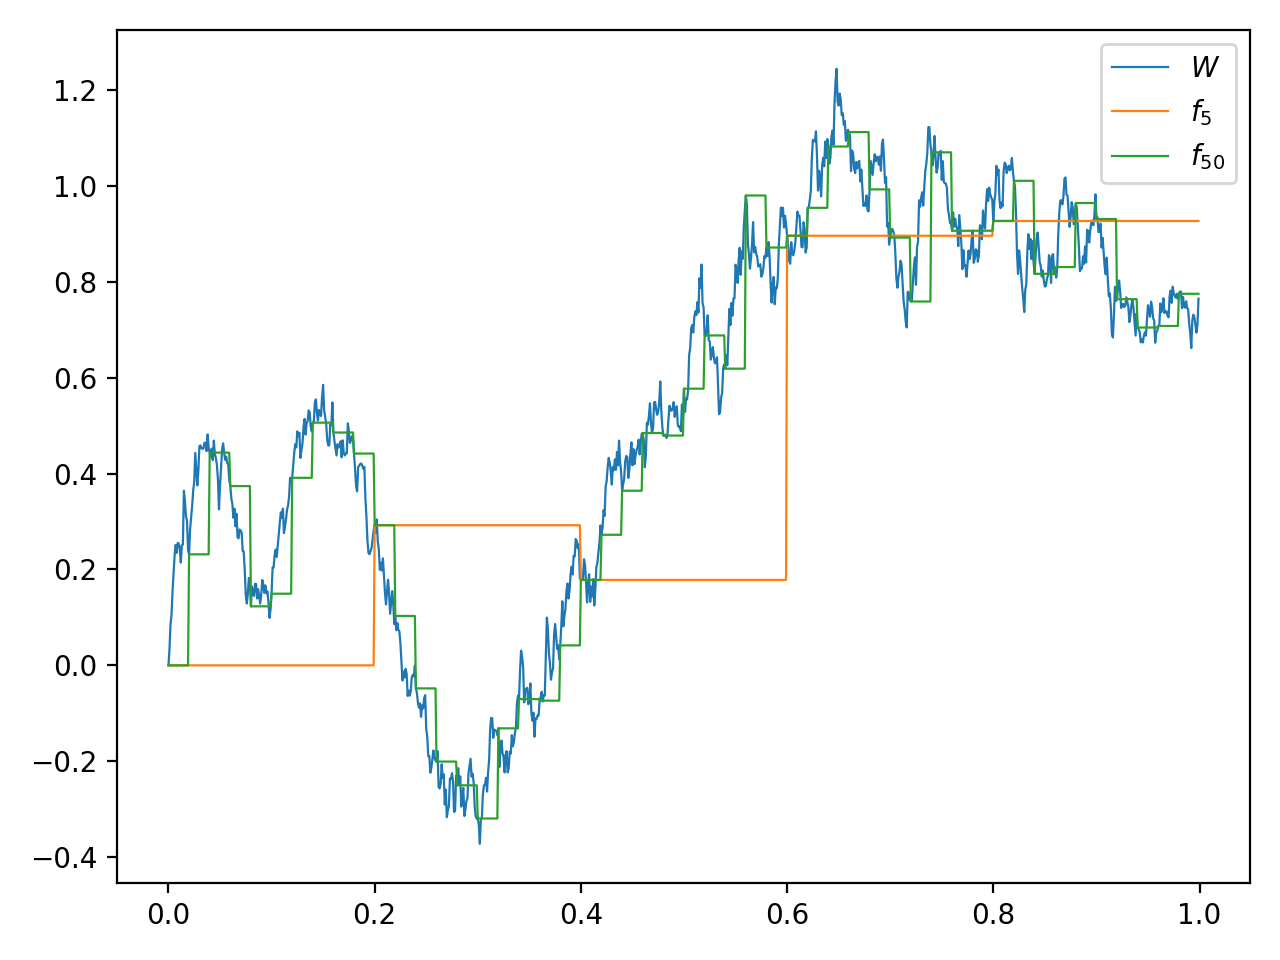
\includegraphics[width=0.9\textwidth]{gfx/21_fig.png}
\caption{Ein typischer Pfad von $f$ und $f_n$}
\end{figure}

\begin{enumerate}
%a
\item $M^2$-Fehler der Approximation von $f$ bestimmen.
\begin{align*}
\norm{f_n-f}{M^2} &= \norm{\sum_{j=0}^{n-1} \left(W(\frac{j}{n})-W(t)\right) \indd{[\frac{j}{n}, \frac{j+1}{n})}(t)}{M^2}\\
&= \Ee{\int \sum_{j=0}^{n-1} \left(W(\frac{j}{n})-W(t)\right)^2 \indd{[\frac{j}{n}, \frac{j+1}{n})}(t) dt}\\
&= \int \Ee{\sum_{j=0}^{n-1} \left(W(\frac{j}{n})-W(t)\right)^2 \indd{[\frac{j}{n}, \frac{j+1}{n})}(t) } dt &\text{Fubini-Tonelli}\\
&= \int \sum_{j=0}^{n-1} \Ee{\left(W(\frac{j}{n})-W(t)\right)^2} \indd{[\frac{j}{n}, \frac{j+1}{n})}(t)  dt\\
&= \int \sum_{j=0}^{n-1} \left(t-\frac{j}{n}\right) \indd{[\frac{j}{n}, \frac{j+1}{n})}(t)  dt & \text{$W$ neu gestartet}\\
&=  \sum_{j=0}^{n-1} \int\left(t-\frac{j}{n}\right) \indd{[\frac{j}{n}, \frac{j+1}{n})}(t)  dt \\
&=  \sum_{j=0}^{n-1} \frac{1}{2n^2} & \text{$\int$ = halbes Quadrat der Länge $\frac{1}{n}$}\\
&= \frac{1}{2n}
\end{align*}
Man beachte, dass mit Itô-Isometrie gilt
$$\frac{1}{2n} = \norm{f_n-f}{M^2} = \norm{I(f_n-f)}{L^2} = \norm{I(f_n)-I(f)}{L^2} = \norm{I(f_n)-Y}{L^2}$$

%b
\item $L^2$-Fehler der Approximation der Itô-Integrale, ohne Isometrie.

In Punkt (a) haben wir schon gezeigt dass $\frac{1}{2n}$ herauskommt, keine Notwendigkeit jetzt in (b) die Isometrie zu bemühen!

Aber gut, rechnen wir zu Fuß. Zuerst mal das Itô-Integral vom Treppenprozess. Um die Lesbarkeit zu verbessern, schreiben wir $W_{j}$ statt $W(\frac{j}{n})$.
$$I(f_n) = \sum_{j=0}^{n-1} W_j \left( W_{j+1} - W_j\right)$$

Jetzt schauen wir uns den gesuchten $L^2$-Abstand an:
\begin{align*}
\norm{I(f_n)-Y}{L^2} &= \Ee{(I(f_n) - Y)^2}\\
&= \Ee{(I(f_n))^2} -2\Ee{(I(f_n)Y} + \Ee{Y^2}
\end{align*}

Erster Term, wir nutzen Unabhängigkeit der Inkremente:
\begin{align*}
\Ee{(I(f_n))^2} &= \Ee{\left(\sum_{j=0}^{n-1} W_j \left( W_{j+1} - W_j\right)\right)^2}\\
&= \Ee{\sum_{j=0}^{n-1} W_j^2 \left( W_{j+1} - W_j\right)^2 + 2 \sum_{j=0}^{n-1} \sum_{k>j}^{n-1} W_j \left( W_{j+1} - W_j\right) \cdot W_k \left( W_{k+1} - W_k\right) }\\
&= \sum_{j=0}^{n-1} \Ee{W_j^2} \Ee{\left( W_{j+1} - W_j\right)^2} + 2 \sum_{j=0}^{n-1} \sum_{k>j}^{n-1} \Ee{W_j \left( W_{j+1} - W_j\right) W_k} \Ee{\left( W_{k+1} - W_k\right)}\\
&=\sum_{j=0}^{n-1} \frac{j}{n} \frac{1}{n} + 2 \sum_{j=0}^{n-1} \sum_{k>j}^{n-1} \Ee{W_j \left( W_{j+1} - W_j\right) W_k} \cdot 0\\
&=\frac{1}{n^2}\sum_{j=0}^{n-1} j\\
&=\frac{1}{n^2}\frac{(n-1)n}{2}\\
&=\frac{1}{2} - \frac{1}{2n}
\end{align*}


Mittlerer Term:
\begin{align*}
\Ee{(I(f_n)Y} &= \Ee{\sum_{j=0}^{n-1} W_j \left( W_{j+1} - W_j\right) \left(\frac{W_n^2-1}{2}\right)}\\
&= \sum_{j=0}^{n-1} \Ee{W_j \left( W_{j+1} - W_j\right) \left(\frac{W_n^2-1}{2}\right)}\\
&= \frac{1}{2}\sum_{j=0}^{n-1} \Ee{W_j \left( W_{j+1} - W_j\right) \left(W_n^2-1\right)}\\
&= \frac{1}{2}\sum_{j=0}^{n-1} \Ee{W_j \left( W_{j+1} - W_j\right) W_n^2} - \Ee{W_j \left( W_{j+1} - W_j\right)}\\
\end{align*}
Wir rechnen die beiden Erwartungswerte in der Summe aus. Der rechte ist einfach, da das Inkrement unabhängig vom Startzeitpunkt ist. Für den linken verwenden wir $\Delta_b W_a := W_{a+b} - W_a$ als Notation für das $\frac{b}{n}$ lange Inkrement von $\frac{a}{n}$ weg.
\begin{align*}
\Ee{W_j \left( W_{j+1} - W_j\right)} &= 0\\
\end{align*}
\begin{align*}
&~~~~ \Ee{W_j \left( W_{j+1} - W_j\right) W_n^2} \\
&= \Ee{W_j (\Delta_1 W_j) W_n^2}\\
&= \Ee{W_j \Delta_1 W_j (\Delta_{n-(j+1)}W_{j+1} + W_{j+1})^2}\\
&= \Ee{W_j \Delta_1 W_j (\Delta_{n-(j+1)}W_{j+1})^2} + &\text{3 unabh. Faktoren}\\
&\hdots + 2 \Ee{W_j \Delta_1 W_j (\Delta_{n-(j+1)}W_{j+1}) W_{j+1}} + &\text{2. Inkrement unabh.}\\
&\hdots + \Ee{W_j \Delta_1 W_j W_{j+1}^2} \\
&= 0 + 0 + \Ee{W_j \Delta_1 W_j W_{j+1}^2} \\
&= \Ee{W_j \Delta_1 W_j (\Delta_1Wj + W_j)^2} \\
&= \Ee{W_j (\Delta_1 W_j)^3} + 2 \Ee{W_j^2 (\Delta_1 W_j)^2} + \Ee{W_j^3 (\Delta_1 W_j)} \\
&= 0 + 2\Vv{W_j}\Vv{\Delta_1 W_j} + 0 \\
&= 2 \frac{j}{n^2}
\end{align*}
Zurück eingesetzt ergibt sich:
\begin{align*}
\Ee{(I(f_n)Y} &= \frac{1}{2}\sum_{j=0}^{n-1} 2 \frac{j}{n^2} - 0 \\
&= \frac{1}{n^2} \cdot \frac{(n-1)n}{2} \\
&= \frac{1}{2} - \frac{1}{2n}
\end{align*}

Hinterster Term:
\begin{align*}
\Ee{Y^2} &= \Ee{\left(\frac{W(1)^2-1}{2}\right)^2}\\
&= \frac{1}{4}\left(\Ee{(W(1))^4} -2\Ee{(W(1))^2}\cdot 1 +1^2\right)\\
&= \frac{1}{4}\left(3\cdot 1^4 -2\cdot 1 +1\right) &\text{Momente}\\
&= \frac{1}{2}
\end{align*}
\end{enumerate}

Insgesamt:
\begin{align*}
\norm{I(f_n)-Y}{L^2} &= \Ee{(I(f_n) - Y)^2}\\
&= \Ee{(I(f_n))^2} -2\Ee{(I(f_n)Y} + \Ee{Y^2}\\
&=\frac{1}{2} - \frac{1}{2n} - 2\cdot\left(\frac{1}{2} - \frac{1}{2n}\right) +\frac{1}{2}\\
&= \frac{1}{2n}
\end{align*}
Mühsam. Ein Hoch auf die Itô-Isometrie.

\newpage
%22
\item Sei
$$g_n(t) := \sum_{j=0}^{n-1} (W(\frac{j}{n}))^2 \indd{[\frac{j}{n}, \frac{j+1}{n})}(t)$$
\begin{enumerate}
%a
\item Varianz des Itô-Integrals ausrechnen.
\begin{align*}
\Vv{I(g_n)} &= \Ee{(I(g_n))^2}\\
&=\Ee{\int g_n^2 dt}\\
&= \int \Ee{g_n^2} dt\\
&= \int \Ee{\sum_{j=0}^{n-1} (W(\frac{j}{n}))^4 \indd{[\frac{j}{n}, \frac{j+1}{n})}(t)} dt\\
&= \int \sum_{j=0}^{n-1} \Ee{(W(\frac{j}{n}))^4} \indd{[\frac{j}{n}, \frac{j+1}{n})}(t) dt\\
&= \int \sum_{j=0}^{n-1} 3(\frac{j}{n})^4 \indd{[\frac{j}{n}, \frac{j+1}{n})}(t) dt &\text{(viertes Moment Normalverteilung)}\\
&= \sum_{j=0}^{n-1} 3(\frac{j}{n})^4 \int \indd{[\frac{j}{n}, \frac{j+1}{n})}(t) dt\\
&= \sum_{j=0}^{n-1} 3(\frac{j}{n})^4 \frac{1}{n} &(*)\\
&= \frac{3}{n^5} \sum_{j=0}^{n-1} j^4 \\
\end{align*}
In der Darstellung $(*)$ steht eine Riemannsumme zum Integral $\int_0^1 3x^4 dx$ mit äquidistanten Stützstellen $x_j = \frac{j}{n} \Rightarrow \Delta x = \frac{1}{n}$, womit diese Summe für $n\rightarrow \infty$ gegen $\left. \frac{3}{5}x^5\right|_0^1 = \frac{3}{5}$ geht.

%b
\item Summen über eine feste Potenz natürlicher Zahlen: Nach wem sind Formeln benannt, die sowas anders darstellen?

\begin{figure}[h!]
\centering
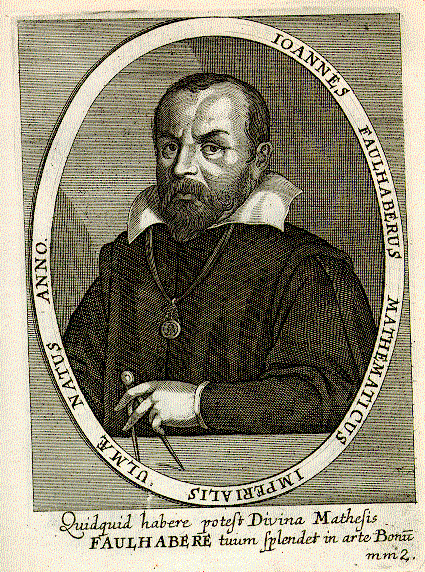
\includegraphics[width=0.5\textwidth]{gfx/Ioannes-Faulhaberus-Mathematicus-Imperialis-Ulmae-Natus.png}
\caption{Johannes Faulhaber}
\end{figure}

\textsc{Johannes Faulhaber}, der in der Spätrenaissance um 1600 herum gelebt hat, hat für $n=1..11$ konkrete Formeln aufgestellt.
Die allgemeine Familie der Identitäten
$$\sum_{j=0}^{n-1} j^k = \frac{1}{k+1}\sum_{j=0}^k \binom{k+1}{j} B_{j} n^{k+1-j} \in \text{\{Polynome in $n$ vom Grad $k+1$\}}$$
wobei $B_j$ die $j$-te Bernoulli-Zahl erster Art bezeichnet, ist daher nach Faulhaber benannt.
Faulhaber war Mathematiker, Ingenieur, Festungsbaumeister (Basel und Frankfurt), Rechnenmeister, Numerologe, Alchemist, Astrologe, Erfinder, ein Freund Keplers.


Die \textsc{Erdős}-\textsc{Moser}-Gleichung hat die Gestalt
$$\sum_{j=0}^{m} j^k = (m+1)^k$$
und ordnet sich damit in die Familie ein. Eine bekannte Lösung lautet $1^1+2^1=3^1$, seit 70 Jahren hat man keine weitere Lösung gefunden, weiß aber dass $m>10^{1000000000}$ gelten müsste.


\begin{figure}[h!]
\centering
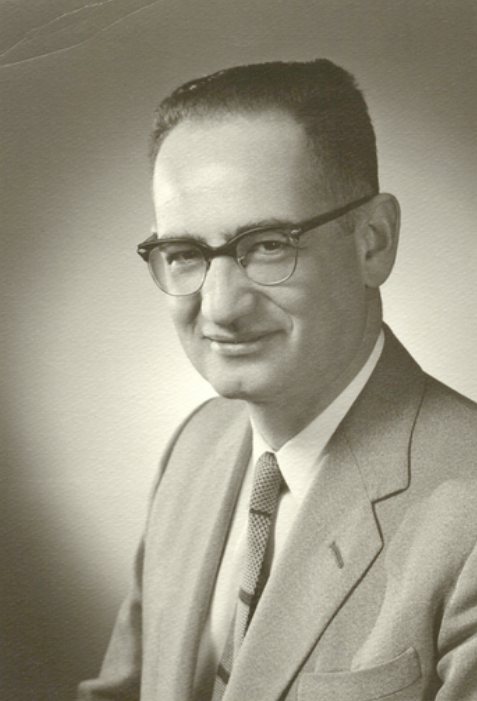
\includegraphics[width=0.5\textwidth]{gfx/Leo_Moser.png}
\caption{Leo Moser}
\end{figure}
\textsc{Leo Moser}, Namensgeber obiger Gleichung, hat übrigens ein weiteres bisher ungelöstes, sehr elegantes Problem formuliert (Moser's worm problem):
\emph{Was ist eine Figur mit minimalem Flächeninhalt in der Ebene, so dass man jede Kurve der Länge $1$ einschreiben kann?}\\
Man weiß dass so eine Figur existieren muss (anders als beim Streichholz-Umdreh-Problem beispielsweise), und seit 2017 auch dass ein Kreissektor, der $\frac{1}{6}$ des Einheitskreises ist, eine obere Schranke bildet.


Zurück zu den Summen: Wenn man $n\rightarrow \infty$ gehen lässt, konvergieren die Summen nicht mehr. Wenn wir aber negative Exponenten zulassen, oder gleich komplexe, dann landen wir schnell bei der Riemannschen Zeta-Funktion:
$$\zeta (z) := \sum_{n=1}^\infty \frac{1}{n^z}$$
Diese Funktion taucht vielerorts prominent auf und ist super wichtig, siehe Literatur.
\end{enumerate}

\newpage
%23
\item Markovkette mit vier Zuständen, Anfangsverteilung $\lambda = (0.5, 0.5, 0, 0)$ und der Übergangsmatrix
$$P=\begin{pmatrix}
\frac{1}{3} & \frac{1}{3} & 0 & \frac{1}{3} \\
\frac{1}{4} & \frac{1}{4} & \frac{1}{4} & \frac{1}{4} \\
0 & 0 & \frac{1}{2} & \frac{1}{2} \\
0 & 0 & 0 & 1
\end{pmatrix}$$
\begin{enumerate}
%a
\item Wir verwenden das Prinzip $\pp{A \wedge B} = \pp{A} \cdot \pp{B|A}$. Wegen der Markoveigenschaft können wir die gesamte Bedingung auf die Bedingung durch den letzten Zeitpunkt runterbrechen. Damit ergibt sich:
\begin{align*}
&\pp{X_0 = 2, X_1 = 1, X_2 = 2, X_3 = 1} \\
=~&\pp{X_0 = 2} \cdot \pp{X_1 = 1 | X_0 = 2} \cdot \pp{X_2 = 2 | X_1 = 1} \cdot \pp{X_3 = 1 | X_2 = 2} \\
=~&\lambda_2 \cdot P_{2, 1} \cdot P_{1, 2} \cdot P_{2, 1} \\
=~&\frac{1}{2} \cdot \frac{1}{4} \cdot \frac{1}{3} \cdot \frac{1}{4} = \frac{1}{96}
\end{align*}
Desweiteren:
\begin{align*}
&\pp{X_0 = 2, X_2 = 2, X_3 = 1} \\
=~&\pp{X_0 = 2} \cdot \pp{X_2 = 2 | X_0 = 2} \cdot \pp{X_3 = 1 | X_2 = 2} \\
=~&\lambda_2 \cdot P^2_{2, 2} \cdot P_{2, 1} \\
=~&\frac{1}{2} \cdot (\frac{1}{3}\frac{1}{4} + \frac{1}{4}\frac{1}{4} + 0 \frac{1}{4}+ 0 \frac{1}{4}) \cdot \frac{1}{4} \\
=~&\frac{1}{2} \cdot \frac{7}{48} \cdot \frac{1}{4}  = \frac{7}{384}\\
\end{align*}

%b
\item Die Kommunikationsklassen sind $\{1, 2\}, \{3\}$ und $\{4\}$. Die ersten Beiden sind transient, die letzte ist rekurrent.

%c
\item Sei $T$ die Stoppzeit um in 1 oder 4 zukommen.
\begin{align*}
\pp{T < \infty} &= 1 \\
\ppp{2}{T = 2} &= \pp{X_1 \in \{2,3\}, X_2 \in \{1,4\} | X_0 = 2} \\
&= \pp{X_1 = 2 | X_0 = 2} \pp{ X_2 \in \{1,4\} | X_1 = 2} + \hdots \\
&\hdots + \pp{X_1 = 3 | X_0 = 2} \pp{ X_2 \in \{1,4\} | X_1 = 3} \\
&= P_{2,2}(P_{2,1}+P_{2,4}) + P_{2,3}(P_{3,1}+P_{3,4}) \\
&= \frac{1}{4} \left(\frac{1}{4} + \frac{1}{4}\right) + \frac{1}{4}\left(0 + \frac{1}{2}\right) \\
&= \frac{1}{8} + \frac{1}{8} = \frac{1}{4}
\end{align*}

%d
\item Mittlere Trefferzeit wie oben aber bei Start in jeweiligen Zuständen ausrechnen.
\begin{align*}
k_1 &= 0 \\
k_4 &= 0 \\
k_3 &= 1 + \frac{k_3 + k_4}{2} = 1 + \frac{k_3}{2} = 2\\
k_2 &= 1 + \frac{k_1 + k_2 + k_3 + k_4}{4} = 1 + \frac{k_2 + 2}{4} = \frac{3}{2} + \frac{k_2}{4} = 2\\
\end{align*}

%e
\item Was ist die Varianz von $T$ unter $\p_3$? Da man vom Zustand 3 nicht zu 1 oder 2 kommt, sind nur die Zustände 3 und 4 relevant. Die Frage ist nun, wie oft man im Zustand 3 bleibt. Das entspricht einer geometrischen Verteilung: $T \sim G\left(\frac{1}{2}\right)$. $$\V_3\left[T\right] = \frac{1-p}{p^2} = \frac{1-\frac{1}{2}}{\frac{1}{2}^2} = 2$$
\begin{align*}
\end{align*}
\end{enumerate}

%24
\item 
\begin{enumerate}
%a
\item Wahrscheinlichkeiten von zwei konkreten Zustandsfolgen:
\begin{align*}
\pp{X_3 = 2, X_2 = 1, X_1 = 0, X_0 = 0} &= \frac{1}{3}\cdot\frac{1}{2}\cdot\frac{1}{2}\cdot\frac{1}{2} = \frac{1}{24} \\
\pp{X_3 = 2, X_2 = 1, X_1 = 0} &= \frac{2}{3}\cdot\frac{1}{2}\cdot\frac{1}{2}\cdot\frac{1}{2} = \frac{1}{12}
\end{align*}

%b
\item Ist diese Kette irreduzibel? Ja, jeder Zustand ist von jedem anderen erreichbar. Für alle Zustände $i, j$ existiert $n = |i-j|$ sodass: $$\pp{X_{|i-j|} = j | X_0 = i} = \frac{1}{2^{|i-j|}} > 0$$

%c
\item Alle Zustände kommunizieren miteinander, siehe (b), deshalb sind alle Trefferzeiten f.s. endlich. In Symbolen: $$\forall i : h_i := \ppp{i}{H < \infty} = 1$$

%d
\item LGS für mittlere Trefferzeiten in $0$:
\begin{align*}
k_0 &= 0 \\
k_1 &= 1 + \frac{k_0 + k_2}{2} \\
k_2 &= 1 + \frac{k_1 + k_3}{2} \\
k_3 &= 1 + \frac{k_2 + k_4}{2} \\
k_4 &= 1 + \frac{k_3 + k_4}{2}
\end{align*}
In Matrixform:
\begin{align*}
\frac{1}{2}
\begin{pmatrix*}[r]
2&-1&0&0 \\
-1&2&-1&0 \\
0&-1&2&-1 \\
0&0&-1&1
\end{pmatrix*} \cdot
\begin{pmatrix}
k_1 \\ k_2 \\ k_3 \\ k_4
\end{pmatrix}
 = 
\begin{pmatrix}
1 \\ 1 \\ 1 \\ 1
\end{pmatrix}
\end{align*}
Das führt zur Lösung $(k_0, k_1, k_2, k_3, k_4) = (0,8,14,18,20)$.
\end{enumerate}

%25
\item Wir spielen ein Münzwurfspiel um Geld, bei dem in jeder Runde unser Kapital um $\pm 1$ je nach Kopf/Zahl verändert wird. Was ist die Wahrscheinlichkeit, bei Startkapital $i$ in endlicher Zeit in den Ruin zu kommen? Wir bedienen uns einer Markovkette und dem zugehörigen LGS.

Für alle $a \in \R$ ist $(h_i := ai + 1)_{i \in \N}$ eine Lösung des LGS:
\begin{align*}
1 &\stackrel{!}{=} h_0 = a\cdot 0 + 1 = 1 \\
h_i &\stackrel{!}{=} \frac{1}{2}h_{i-1} + \frac{1}{2}h_{h+1} \\
&= \frac{1}{2}(a(i-1) + 1 + a(i+1) + 1)) \\
&= \frac{1}{2}(2ai + 2) \\
&= ai+1 = h_i
\end{align*}
Damit haben wir unendlich viele Lösungen. Das sind auch schon alle, denn $h_0 = 1$ ist fest, und $a := h_1 - 1$ berechnet sich aus $h_1$. Höhere $h_i$ für $i>1$ sind dann durch Induktion und die zweite Gleichung eindeutig bestimmt.

Für $a < 0$ ergeben sich $h_i < 0$ für große $i$\footnote{Jargon-Warnung: Weil $\R$ ein archimedischer Körper ist.}, also kann $h_i$ wohl keine Wahrscheinlichkeit sein. Analog, für $a > 0$ ist $h_1 > 1$, also kann es auch keine Wahrscheinlichkeit sein. Nur $a = 0$ und damit $h_i = 1$ bleibt als Möglichkeit übrig.

\end{enumerate}












\end{document}
